%please update these for each book release:

\newcommand{\bookauthor}{J. W. Milnor and J. D. Stasheff}
\newcommand{\shortbookauthor}{Milnor and Stasheff}
\newcommand{\booktitle}{Characteristic Classes}
\newcommand{\booksubtitle}{}

\newcommand{\bookcoverTeXromancers}{Revised and modernized edition by}

\newcommand{\bookcoverpicture}{
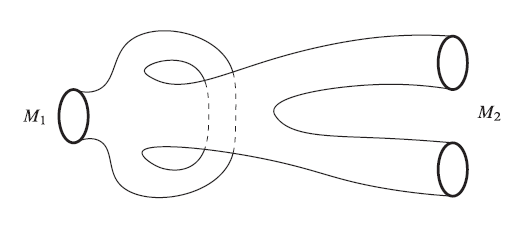
\includegraphics[height=21em]{./fig6.PNG}
}

\newcommand{\bookoriginaledition}{1965}
\newcommand{\bookthisedition}{2022}

%these are meant for the back cover
%both should have ~100 words
\newcommand{\bookreview} 
{The theory of characteristic classes provides a meeting ground for the various disciplines of differential topology, differential and algebraic geometry, cohomology, and fiber bundle theory. As such, it is a fundamental and an essential tool in the study of differentiable manifolds.
\\[1em]

In this volume, the authors provide a thorough introduction to characteristic classes, with detailed studies of Stiefel-Whitney classes, Chern classes, Pontrjagin classes, and the Euler class. Three appendices cover the basics of cohomology theory and the differential forms approach to characteristic classes, and provide an account of Bernoulli numbers.
\\[1em]

Based on lecture notes of John Milnor, which first appeared at Princeton University in 1957 and have been widely studied by graduate students of topology ever since.
}

\newcommand{\bookauthorbio}
{Awards and Recognition
\\[1em]

\defemph{John Milnor}, Winner of the 2011 Abel Prize from the Norwegian Academy of Science and Letters
\\[1em] Winner of the 2011 Leroy P. Steele Prize for Lifetime Achievement, American Mathematical Society
}
\newcommand{\authorbiosource}{Princeton press} 